\documentclass[11pt]{article}
\usepackage{euscript}

\usepackage{amsmath}
\usepackage{amsthm}
\usepackage{amssymb}
\usepackage{epsfig}
\usepackage{xspace}
\usepackage{color}
\usepackage{url}

%%%%%%%%%%%%%%%%%%%%%%%%%%%%%%%%%
\setlength{\textheight}{9in}
\setlength{\topmargin}{-0.600in}
\setlength{\headheight}{0.2in}
\setlength{\headsep}{0.250in}
\setlength{\footskip}{0.5in}
\flushbottom
\setlength{\textwidth}{6.5in}
\setlength{\oddsidemargin}{0in}
\setlength{\evensidemargin}{0in}
\setlength{\columnsep}{2pc}
\setlength{\parindent}{1em}
%%%%%%%%%%%%%%%%%%%%%%%%%%%%%%%%%


\newcommand{\eps}{\varepsilon}

\renewcommand{\c}[1]{\ensuremath{\EuScript{#1}}}
\renewcommand{\b}[1]{\ensuremath{\mathbb{#1}}}
\newcommand{\s}[1]{\textsf{#1}}

\newcommand{\E}{\textbf{\textsf{E}}}
\renewcommand{\Pr}{\textbf{\textsf{Pr}}}

\title{HW03: Game Playing
\footnote{\s{CS 5300 AI; \;\; Spring 2012 \hfill
Instructor: Jur van den Berg, University of Utah}
}
}
\author{Alex Clemmer, u0458675}

\begin{document}
\maketitle





%%%%%%%%%%%%%%%%%%%%%%%%%%%%%%%%%%%%%%%%%%%%%%%%%%%%
%%%%%%%%%%%%%%%%%%%%%%%%%%%%%%%%%%%%%%%%%%%%%%%%%%%%
%%%%%%%%%%%%%%%%%%%%%%%%%%%%%%%%%%%%%%%%%%%%%%%%%%%%
\section{Game Trees \& Minimax}

I have drawn \textbf{a.} and \textbf{b.} simultaneously. Initial values indicated in \textbf{blue}; backed up minimax indicated in \textbf{red}.

\begin{center}
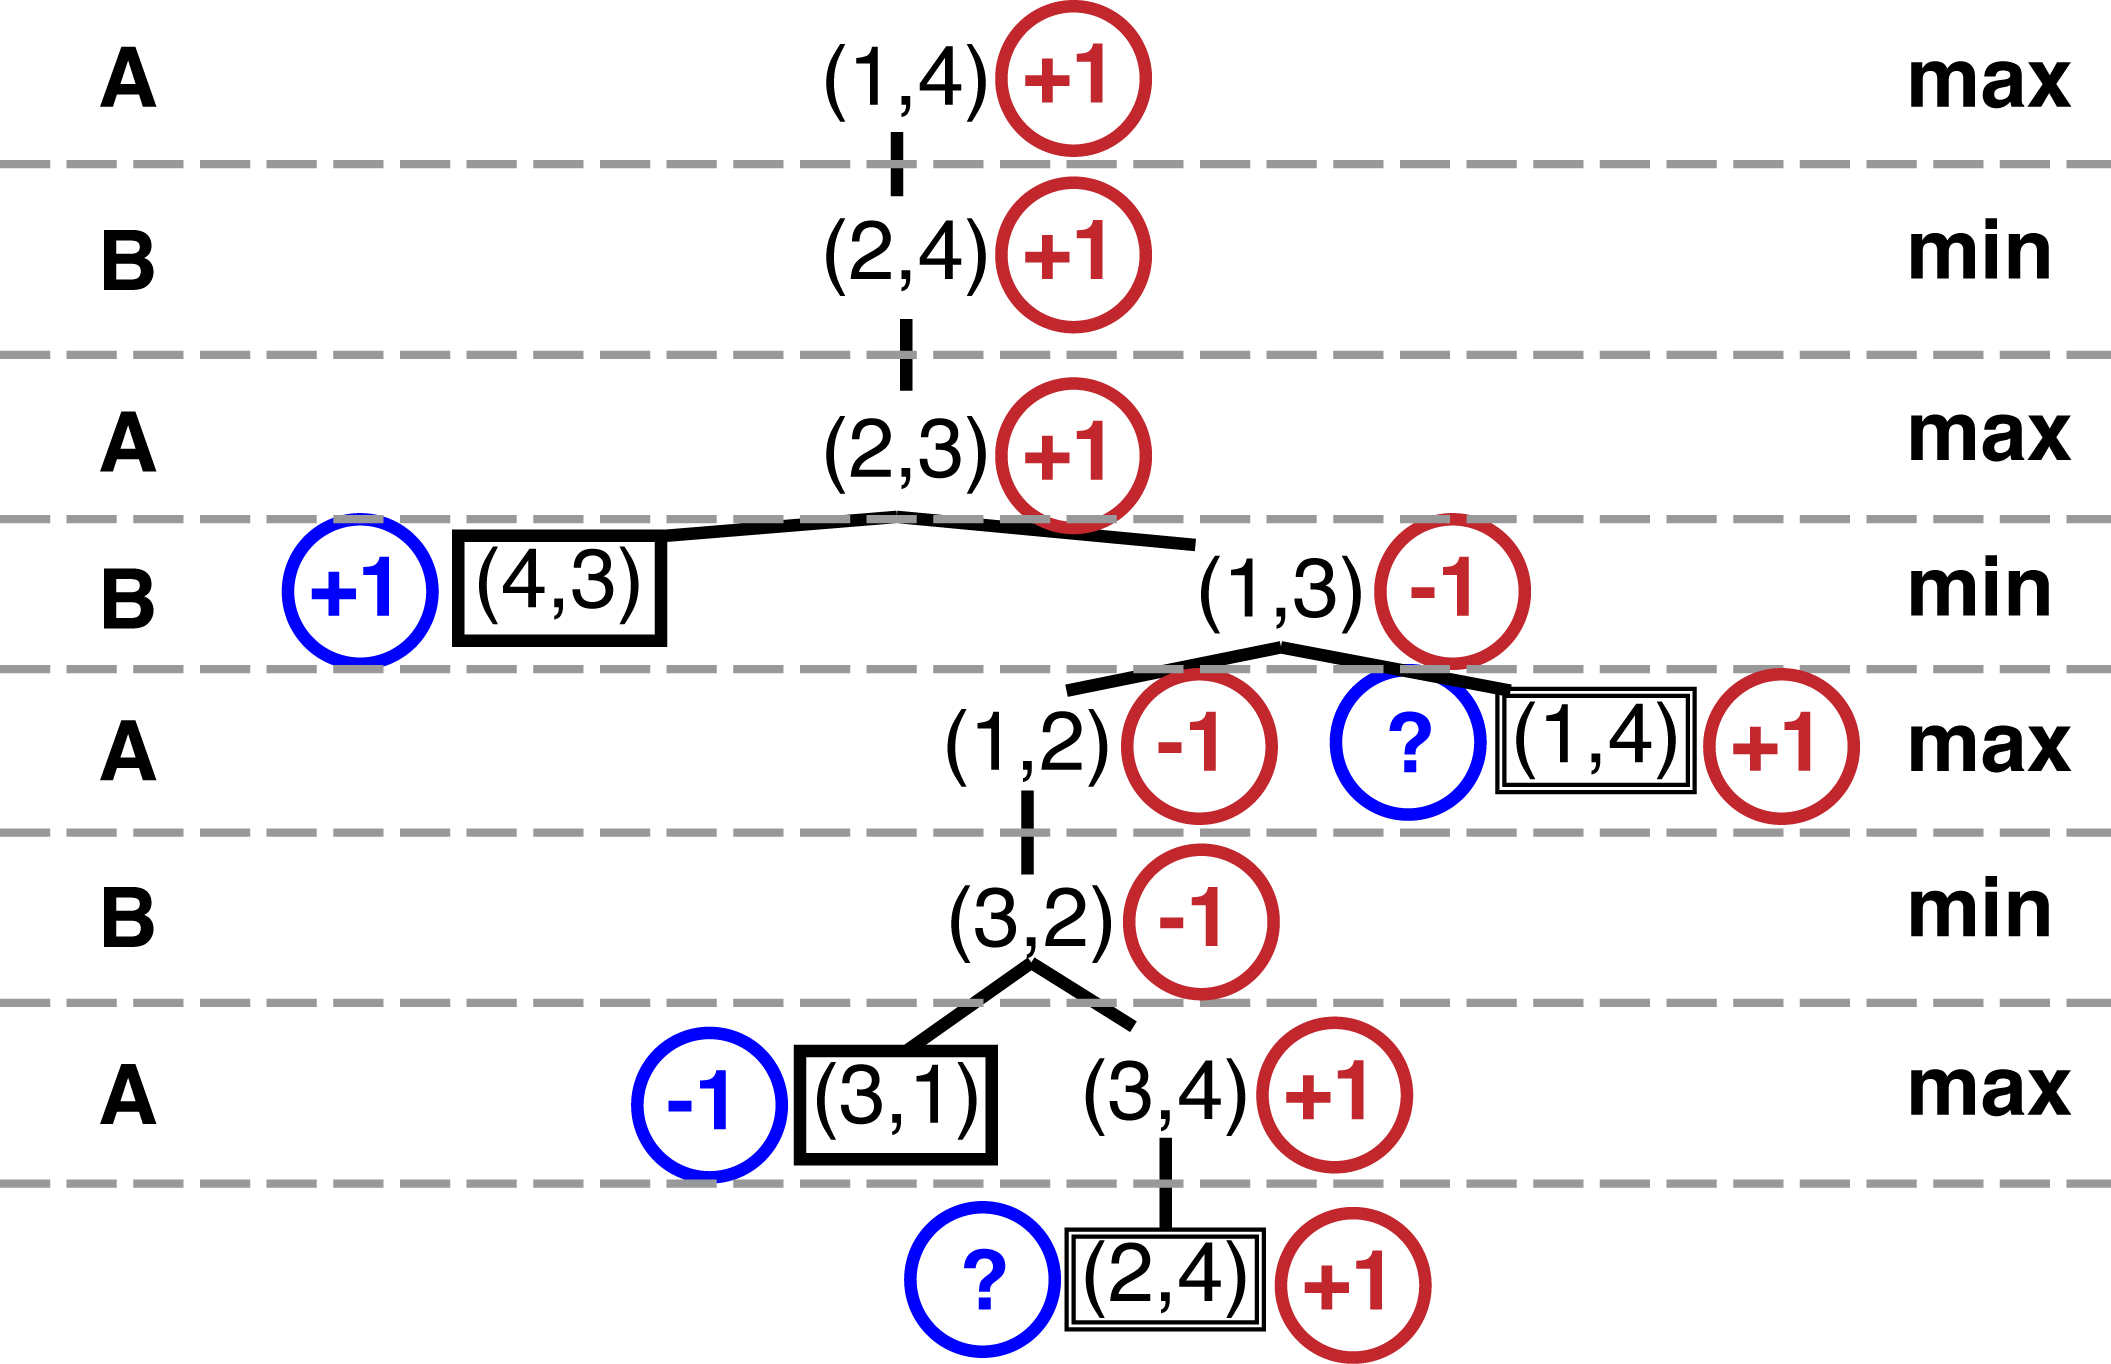
\includegraphics[scale=0.5]{tree.png}
\end{center}

There are two positions that are maked with a `?'. Because these states occurred previously in the tree, and the moves available are exactly the same. So I have annotated them with the same values. This is not actually uncommon---Markov chains are often infinitely recursive as well.


\section{More Minimax}

n/a




\section{Unfair Wagers}

\begin{center}
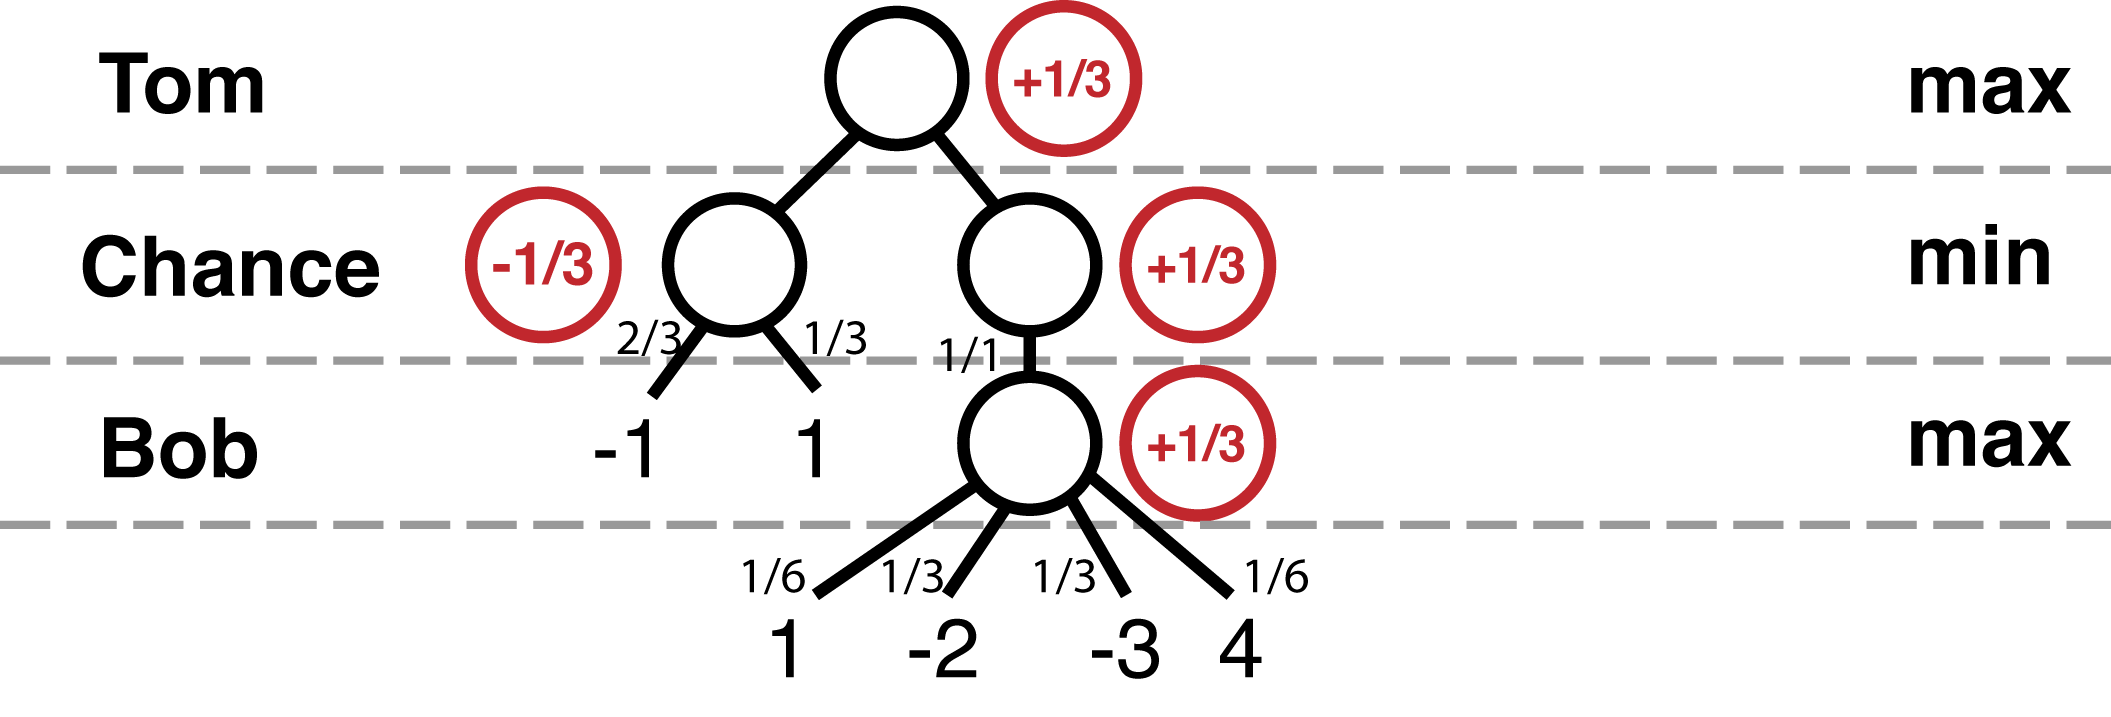
\includegraphics[scale=0.5]{stoc.png}
\end{center}

\textbf{3.} Changing the number 4 to the number 3 makes the expected outcome of that particular node $1 \cdot \frac{1}{6} -2 \cdot \frac{1}{3} - 3 \cdot \frac{1}{6} + 3 \cdot \frac{1}{3} = 0$; changing the 4 to a 2 changes the expected outcome to $1 \cdot \frac{1}{6} -2 \cdot \frac{1}{3} - 3 \cdot \frac{1}{6} + 2 \cdot \frac{1}{3} = - \frac{1}{3}$.

Thus, in order for Bob to con his friend out of his soda (in expectation at least), the number we'd like to change 4 into is \textbf{2}.














\end{document}
